% ============================================================
%  DesignDen – Wireframes & UI Documentation  (LaTeX)
%  Compile with:  pdflatex wireframes.tex
%  Requires: geometry, tikz, xcolor, booktabs, array,
%            fontenc, hyperref, listings, mdframed, tabularx
% ============================================================
\documentclass[a4paper,11pt]{article}

% ── Packages ────────────────────────────────────────────────
\usepackage[a4paper, margin=2cm, top=2.5cm, bottom=2.5cm]{geometry}
\usepackage[T1]{fontenc}
\usepackage{booktabs}
\usepackage[table]{xcolor}
\usepackage{array}
\usepackage{tabularx}
\usepackage{hyperref}
\usepackage{tikz}
\usetikzlibrary{shapes.geometric, arrows, positioning, fit, calc, shadows}
\usepackage{listings}
\usepackage{parskip}
\usepackage{titlesec}
\usepackage{fancyhdr}
\usepackage{mdframed}
\usepackage{enumitem}
\usepackage{multirow}
\usepackage{longtable}
\usepackage{calc}

% ── Colours ─────────────────────────────────────────────────
\definecolor{primary}{HTML}{667eea}
\definecolor{secondary}{HTML}{764ba2}
\definecolor{success}{HTML}{4CAF50}
\definecolor{warning}{HTML}{FFC107}
\definecolor{danger}{HTML}{F44336}
\definecolor{info}{HTML}{2196F3}
\definecolor{dark}{HTML}{1a202c}
\definecolor{muted}{HTML}{718096}
\definecolor{lightbg}{HTML}{f7f8ff}
\definecolor{tabhead}{HTML}{e8eaf6}
\definecolor{rowodd}{HTML}{f3f4ff}
\definecolor{roweven}{HTML}{ffffff}
\definecolor{navbg}{HTML}{16213e}
\definecolor{framebg}{HTML}{1a1a2e}

% ── Hyperref ─────────────────────────────────────────────────
\hypersetup{
  colorlinks=true,
  linkcolor=primary,
  urlcolor=primary,
  pdftitle={DesignDen Wireframes},
  pdfauthor={DesignDen Team},
}

% ── Section titling ──────────────────────────────────────────
\titleformat{\section}{\large\bfseries\color{primary}}{}{0em}{}[\titlerule]
\titleformat{\subsection}[block]{\normalsize\bfseries\color{secondary}}{}{0em}{\colorbox{secondary!10}{\parbox{\dimexpr\linewidth-2\fboxsep}{\strut#1\strut}}}
\titleformat{\subsubsection}{\small\bfseries\color{dark}}{}{0em}{}

% ── Header/Footer ────────────────────────────────────────────
\pagestyle{fancy}
\fancyhf{}
\lhead{\textcolor{primary}{\textbf{DesignDen}} \textcolor{muted}{-- Wireframes \& UI}}
\rhead{\textcolor{muted}{\small v1.0 $\cdot$ March 2026}}
\cfoot{\textcolor{muted}{\thepage}}
\renewcommand{\headrulewidth}{0.4pt}

% ── Column types ─────────────────────────────────────────────
\newcolumntype{L}[1]{>{\raggedright\arraybackslash}p{#1}}
\newcolumntype{C}[1]{>{\centering\arraybackslash}p{#1}}

% ── TikZ: reusable wireframe elements ───────────────────────

% Navbar
\newcommand{\navbar}[2]{%
  \begin{tikzpicture}
    \filldraw[fill=navbg, draw=primary!40] (0,0) rectangle (#1, 0.6);
    \node[anchor=west, font=\small\bfseries, text=primary] at (0.2,0.3) {DesignDen};
    \node[anchor=east, font=\tiny, text=white!70] at (#1-0.15, 0.3) {#2};
  \end{tikzpicture}
}

% Generic screen frame
\newenvironment{wireframe}[2][14cm]{%
  \begin{mdframed}[
    linecolor=primary!60,
    linewidth=1.2pt,
    roundcorner=6pt,
    backgroundcolor=framebg!10,
    innerleftmargin=0pt, innerrightmargin=0pt,
    innertopmargin=0pt, innerbottommargin=6pt
  ]
  \noindent\colorbox{dark}{\parbox{\linewidth}{%
    \hspace{6pt}\textcolor{danger}{$\bullet$}\hspace{2pt}%
    \textcolor{warning}{$\bullet$}\hspace{2pt}%
    \textcolor{success}{$\bullet$}\hspace{10pt}%
    \textcolor{muted}{\small\ttfamily #2}%
  }}\par\vspace{4pt}
}{%
  \end{mdframed}
}

% Button
\newcommand{\wfbtn}[2][primary]{\colorbox{#1!80}{\textcolor{white}{\tiny\textbf{#2}}}}

% ── Listings (code) ───────────────────────────────────────────
\lstset{
  basicstyle=\ttfamily\scriptsize,
  backgroundcolor=\color{lightbg},
  frame=single,
  rulecolor=\color{primary!40},
  breaklines=true,
  keywordstyle=\color{primary}\bfseries,
  commentstyle=\color{muted}\itshape,
  stringstyle=\color{success},
}

% ─────────────────────────────────────────────────────────────
\begin{document}

% ── Title Page ───────────────────────────────────────────────
\begin{titlepage}
  \centering
  \vspace*{2cm}
  {\Huge\bfseries\textcolor{primary}{DesignDen}\par}
  \vspace{0.4cm}
  {\large\textcolor{secondary}{Custom Clothing E-Commerce Platform}\par}
  \vspace{1.5cm}
  \begin{mdframed}[linecolor=primary,linewidth=2pt,innertopmargin=16pt,innerbottommargin=16pt]
    \centering
    {\LARGE\bfseries Wireframes \& UI Documentation}\par
    \vspace{0.3cm}
    {\normalsize 9 Screen Layouts $\cdot$ 5 User Roles $\cdot$ Mobile-First}\par
    \vspace{0.3cm}
    {\small Bootstrap 5.3.8 $\cdot$ Custom CSS $\cdot$ Material Design Inspired}
  \end{mdframed}
  \vspace{2cm}
  \begin{tabular}{rl}
    \textbf{UI Framework} & Bootstrap 5.3.8 + Custom CSS \\[4pt]
    \textbf{Design System}& Material Design Inspired     \\[4pt]
    \textbf{Responsive}   & Mobile-First Approach        \\[4pt]
    \textbf{Version}      & 1.0                          \\[4pt]
    \textbf{Date}         & March 2026                   \\
  \end{tabular}
  \vfill
  {\small\textcolor{muted}{DesignDen Development Team}}
\end{titlepage}

\tableofcontents
\newpage

% ─────────────────────────────────────────────────────────────
\section{Design System Overview}

\subsection{Project Meta}

\rowcolors{2}{rowodd}{roweven}
\begin{tabular}{@{}L{4cm}L{9cm}@{}}
\toprule
\rowcolor{tabhead}
\textbf{Property} & \textbf{Value} \\
\midrule
Project        & DesignDen -- Custom Clothing E-Commerce \\
UI Framework   & Bootstrap 5.3.8 + Custom CSS            \\
Design System  & Material Design Inspired                \\
Approach       & Mobile-First, Responsive                \\
Screens        & 9 unique screen layouts                 \\
User Roles     & 5 (customer, designer, manager, admin, delivery) \\
\bottomrule
\end{tabular}

\subsection{Colour Palette}

\begin{center}
\begin{tikzpicture}
  \foreach \col/\name/\hex [count=\i from 0] in {
    667eea/Primary/\#667eea,
    764ba2/Secondary/\#764ba2,
    4CAF50/Success/\#4CAF50,
    FF9800/Warning/\#FF9800,
    F44336/Danger/\#F44336,
    2196F3/Info/\#2196F3
  }{
    \filldraw[fill={\col}, draw=white] (\i*2.2, 0) rectangle ++(1.8, 0.9);
    \node[font=\tiny\bfseries, text=white, anchor=south west] at (\i*2.2+0.05, 0.48) {\name};
    \node[font=\tiny\ttfamily, text=white!80, anchor=north west] at (\i*2.2+0.05, 0.45) {\hex};
  }
\end{tikzpicture}
\end{center}

\begin{center}
\begin{tikzpicture}
  \foreach \col/\name/\hex [count=\i from 0] in {
    FFC107/Pending/\#FFC107,
    2196F3/In\ Progress/\#2196F3,
    4CAF50/Completed/\#4CAF50,
    F44336/Cancelled/\#F44336,
    00BCD4/Approved/\#00BCD4,
    FF5722/Rejected/\#FF5722
  }{
    \filldraw[fill={\col}, draw=white] (\i*2.2, 0) rectangle ++(1.8, 0.9);
    \node[font=\tiny\bfseries, text=white, anchor=south west] at (\i*2.2+0.05, 0.48) {\name};
    \node[font=\tiny\ttfamily, text=white!80, anchor=north west] at (\i*2.2+0.05, 0.45) {\hex};
  }
\end{tikzpicture}
\end{center}

\subsection{Responsive Breakpoints}

\rowcolors{2}{rowodd}{roweven}
\begin{tabular}{@{}C{1.5cm}C{4cm}L{7cm}@{}}
\toprule
\rowcolor{tabhead}
\textbf{Token} & \textbf{Width Range} & \textbf{Target Device} \\
\midrule
xs & 0px -- 575px   & Mobile (portrait) \\
sm & 576px -- 767px & Large mobile / small tablet \\
md & 768px -- 991px & Tablet \\
lg & 992px -- 1199px& Desktop \\
xl & 1200px -- 1399px& Large Desktop \\
xxl & 1400px+       & Extra Large Desktop \\
\bottomrule
\end{tabular}

% ─────────────────────────────────────────────────────────────
\section{Screen Layouts}

% ─── Screen 1 ────────────────────────────────────────────────
\subsection{Screen 1 — Home Page (Landing)}

\begin{wireframe}{designden.com}

\begin{center}
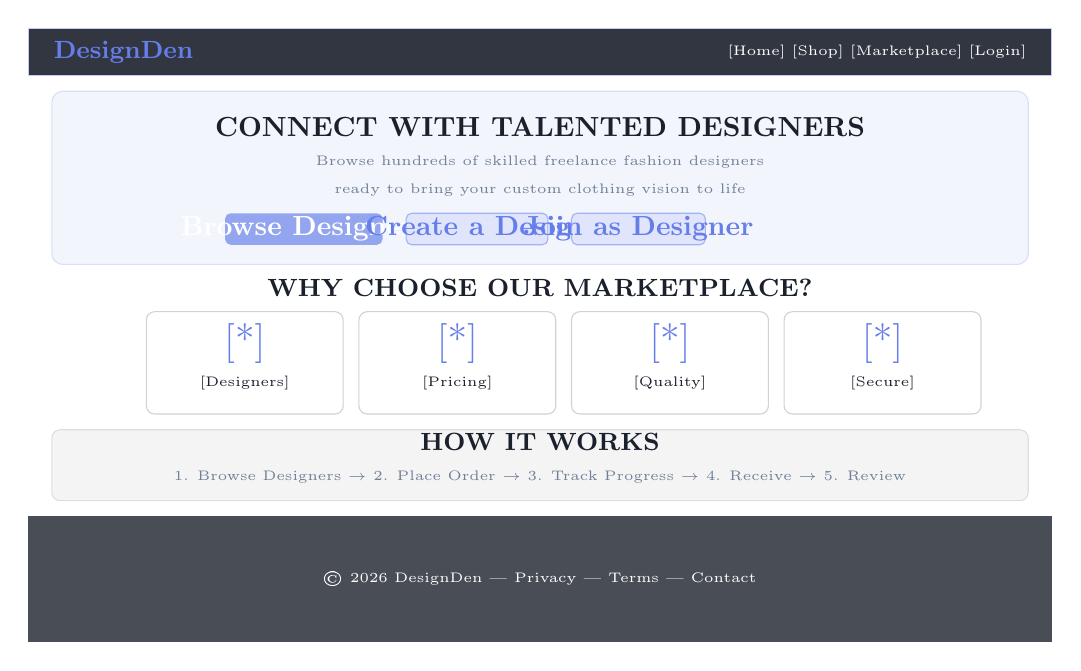
\begin{tikzpicture}[every node/.style={font=\tiny}]
  % Nav
  \filldraw[fill=dark!90, draw=primary!40] (0,7.2) rectangle (13,7.8);
  \node[anchor=west, text=primary, font=\small\bfseries] at (0.2,7.5) {DesignDen};
  \node[anchor=east, text=white!70] at (12.8,7.5) {[Home] [Shop] [Marketplace] [Login]};

  % Hero
  \filldraw[fill=primary!8, draw=primary!25, rounded corners=4pt] (0.3,4.8) rectangle (12.7,7.0);
  \node[font=\normalsize\bfseries, text=dark] at (6.5, 6.55) {CONNECT WITH TALENTED DESIGNERS};
  \node[text=muted, align=center] at (6.5, 6.1) {Browse hundreds of skilled freelance fashion designers};
  \node[text=muted] at (6.5, 5.75) {ready to bring your custom clothing vision to life};
  \filldraw[fill=primary!70, draw=none, rounded corners=2pt] (2.5,5.05) rectangle (4.5,5.45);
  \node[text=white, font=\bfseries] at (3.5,5.25) {Browse Designers};
  \filldraw[fill=primary!20, draw=primary!60, rounded corners=2pt] (4.8,5.05) rectangle (6.6,5.45);
  \node[text=primary, font=\bfseries] at (5.7,5.25) {Create a Design};
  \filldraw[fill=primary!20, draw=primary!60, rounded corners=2pt] (6.9,5.05) rectangle (8.6,5.45);
  \node[text=primary, font=\bfseries] at (7.75,5.25) {Join as Designer};

  % Why section
  \node[font=\small\bfseries, text=dark] at (6.5,4.5) {WHY CHOOSE OUR MARKETPLACE?};
  \foreach \x/\icon/\lbl in {1.5/Talented\,Designers/[Designers], 4.2/Fair\,Pricing/[Pricing],
                               6.9/Quality\,Guaranteed/[Quality], 9.6/Secure\,Payments/[Secure]}{
    \filldraw[fill=white, draw=dark!20, rounded corners=3pt] (\x,2.9) rectangle (\x+2.5,4.2);
    \node[text=primary, font=\Large] at (\x+1.25, 3.8) {[*]};
    \node[text=dark, align=center, font=\tiny] at (\x+1.25, 3.3) {\lbl};
  }

  % How it works
  \filldraw[fill=dark!5, draw=dark!15, rounded corners=3pt] (0.3,1.8) rectangle (12.7,2.7);
  \node[font=\small\bfseries, text=dark] at (6.5,2.55) {HOW IT WORKS};
  \node[text=muted] at (6.5,2.1)
    {1. Browse Designers $\to$ 2. Place Order $\to$ 3. Track Progress $\to$ 4. Receive $\to$ 5. Review};

  % Footer
  \filldraw[fill=dark!80, draw=none] (0,0) rectangle (13,1.6);
  \node[text=white!50, font=\tiny] at (6.5,0.8) {\copyright\ 2026 DesignDen | Privacy | Terms | Contact};
\end{tikzpicture}
\end{center}
\end{wireframe}

% ─── Screen 2 ────────────────────────────────────────────────
\subsection{Screen 2 — 3D Design Studio}

\begin{wireframe}{designden.com/studio}
\begin{center}
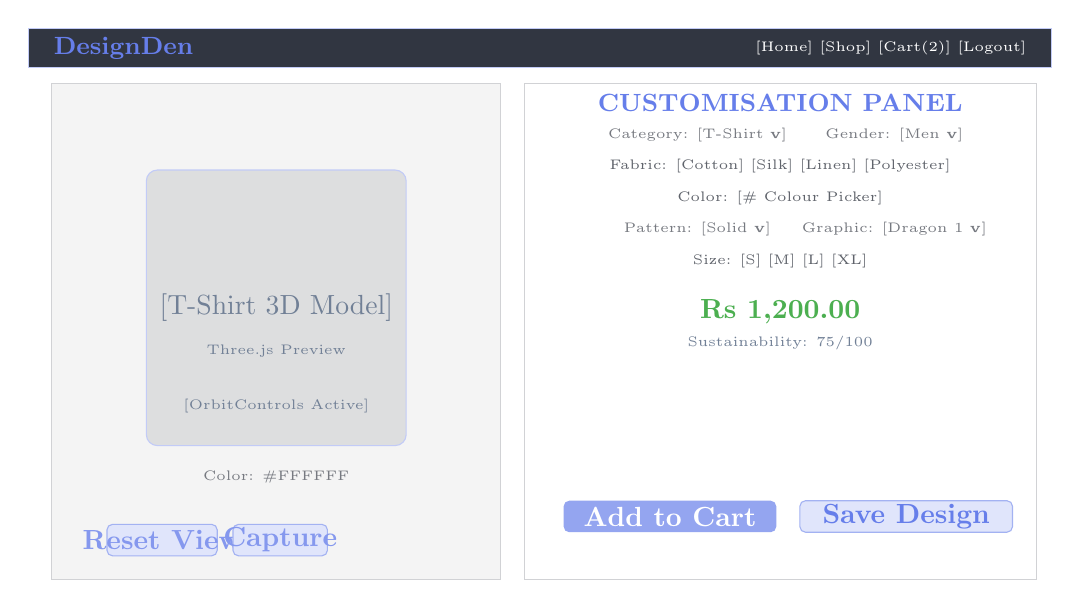
\begin{tikzpicture}[every node/.style={font=\tiny}]
  % Nav
  \filldraw[fill=dark!90, draw=primary!40] (0,6.8) rectangle (13,7.3);
  \node[anchor=west, text=primary, font=\small\bfseries] at (0.2,7.05) {DesignDen};
  \node[anchor=east, text=white!70] at (12.8,7.05) {[Home] [Shop] [Cart(2)] [Logout]};

  % 3D panel
  \filldraw[fill=dark!5, draw=dark!20] (0.3,0.3) rectangle (6.0,6.6);
  \filldraw[fill=dark!15, draw=primary!40, rounded corners=4pt] (1.5,2.0) rectangle (4.8,5.5);
  \node[text=muted, font=\normalsize] at (3.15,3.75) {[T-Shirt 3D Model]};
  \node[text=muted] at (3.15,3.2) {Three.js Preview};
  \node[text=muted] at (3.15,2.5) {[OrbitControls Active]};
  \node[text=dark!60] at (3.15,1.6) {Color: \#FFFFFF};
  \filldraw[fill=primary!20, draw=primary!60, rounded corners=2pt] (1.0,0.6) rectangle (2.4,1.0);
  \node[text=primary!80, font=\bfseries] at (1.7,0.8) {Reset View};
  \filldraw[fill=primary!20, draw=primary!60, rounded corners=2pt] (2.6,0.6) rectangle (3.8,1.0);
  \node[text=primary!80, font=\bfseries] at (3.2,0.8) {Capture};

  % Customisation panel
  \filldraw[fill=white, draw=dark!20] (6.3,0.3) rectangle (12.8,6.6);
  \node[font=\small\bfseries, text=primary] at (9.55,6.35) {CUSTOMISATION PANEL};
  \node[text=dark!60] at (8.5,5.95) {Category: [T-Shirt \textbf{v}]};
  \node[text=dark!60] at (11.0,5.95) {Gender: [Men \textbf{v}]};
  \node[text=dark!70] at (9.55,5.55) {Fabric: [Cotton] [Silk] [Linen] [Polyester]};
  \node[text=dark!70] at (9.55,5.15) {Color: [\# Colour Picker]};
  \node[text=dark!60] at (8.5,4.75) {Pattern: [Solid \textbf{v}]};
  \node[text=dark!60] at (11.0,4.75) {Graphic: [Dragon 1 \textbf{v}]};
  \node[text=dark!70] at (9.55,4.35) {Size: [S] [M] [L] [XL]};
  \node[font=\normalsize\bfseries, text=success] at (9.55,3.7) {Rs 1,200.00};
  \node[text=muted] at (9.55,3.3) {Sustainability: 75/100};
  \filldraw[fill=primary!70, draw=none, rounded corners=2pt] (6.8,0.9) rectangle (9.5,1.3);
  \node[text=white, font=\bfseries] at (8.15,1.1) {Add to Cart};
  \filldraw[fill=primary!20, draw=primary!60, rounded corners=2pt] (9.8,0.9) rectangle (12.5,1.3);
  \node[text=primary, font=\bfseries] at (11.15,1.1) {Save Design};
\end{tikzpicture}
\end{center}
\end{wireframe}

% ─── Screen 3 ────────────────────────────────────────────────
\subsection{Screen 3 — Shopping Cart}

\begin{wireframe}{designden.com/cart}
\begin{center}
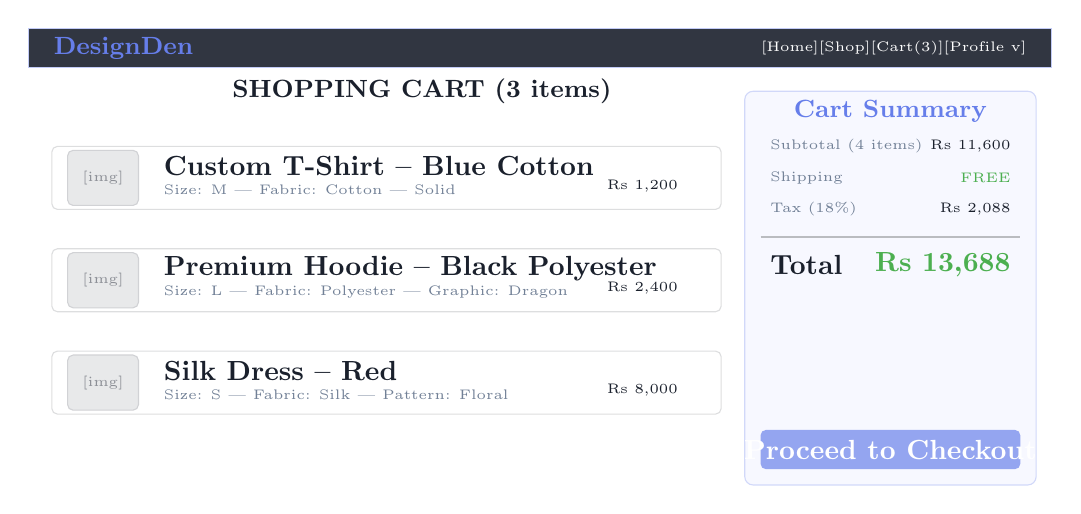
\begin{tikzpicture}[every node/.style={font=\tiny}]
  \filldraw[fill=dark!90, draw=primary!40] (0,6.8) rectangle (13,7.3);
  \node[anchor=west, text=primary, font=\small\bfseries] at (0.2,7.05) {DesignDen};
  \node[anchor=east, text=white!70] at (12.8,7.05) {[Home][Shop][Cart(3)][Profile v]};

  \node[font=\small\bfseries, text=dark] at (5,6.5) {SHOPPING CART (3 items)};

  % Cart items
  \foreach \y/\emoji/\name/\meta in {
    5.5/T-Shirt/Custom T-Shirt -- Blue Cotton/Size: M | Fabric: Cotton | Solid,
    4.2/Hoodie/Premium Hoodie -- Black Polyester/Size: L | Fabric: Polyester | Graphic: Dragon,
    2.9/Dress/Silk Dress -- Red/Size: S | Fabric: Silk | Pattern: Floral
  }{
    \filldraw[fill=white, draw=dark!15, rounded corners=2pt] (0.3,\y-0.5) rectangle (8.8,\y+0.3);
    \filldraw[fill=dark!10, draw=dark!20, rounded corners=2pt] (0.5,\y-0.45) rectangle (1.4,\y+0.25);
    \node[text=dark!50] at (0.95,\y-0.1) {[img]};
    \node[anchor=west, text=dark, font=\bfseries] at (1.6,\y+0.05) {\name};
    \node[anchor=west, text=muted] at (1.6,\y-0.25) {\meta};
  }
  \node[text=dark] at (7.8,5.3) {Rs 1,200};
  \node[text=dark] at (7.8,4.0) {Rs 2,400};
  \node[text=dark] at (7.8,2.7) {Rs 8,000};

  % Summary box
  \filldraw[fill=lightbg, draw=primary!30, rounded corners=3pt] (9.1,1.5) rectangle (12.8,6.5);
  \node[font=\small\bfseries, text=primary] at (10.95,6.25) {Cart Summary};
  \node[text=muted, anchor=west] at (9.3,5.8) {Subtotal (4 items)};
  \node[text=dark, anchor=east] at (12.6,5.8) {Rs 11,600};
  \node[text=muted, anchor=west] at (9.3,5.4) {Shipping};
  \node[text=success, anchor=east] at (12.6,5.4) {FREE};
  \node[text=muted, anchor=west] at (9.3,5.0) {Tax (18\%)};
  \node[text=dark, anchor=east] at (12.6,5.0) {Rs 2,088};
  \draw[dark!30, thick] (9.3,4.65) -- (12.6,4.65);
  \node[text=dark, font=\bfseries, anchor=west] at (9.3,4.3) {Total};
  \node[text=success, font=\bfseries, anchor=east] at (12.6,4.3) {Rs 13,688};
  \filldraw[fill=primary!70, draw=none, rounded corners=2pt] (9.3,1.7) rectangle (12.6,2.2);
  \node[text=white, font=\bfseries] at (10.95,1.95) {Proceed to Checkout};
\end{tikzpicture}
\end{center}
\end{wireframe}

% ─── Screen 4 ────────────────────────────────────────────────
\subsection{Screen 4 — Checkout Page}

\begin{wireframe}{designden.com/checkout (Secure)}
\begin{center}
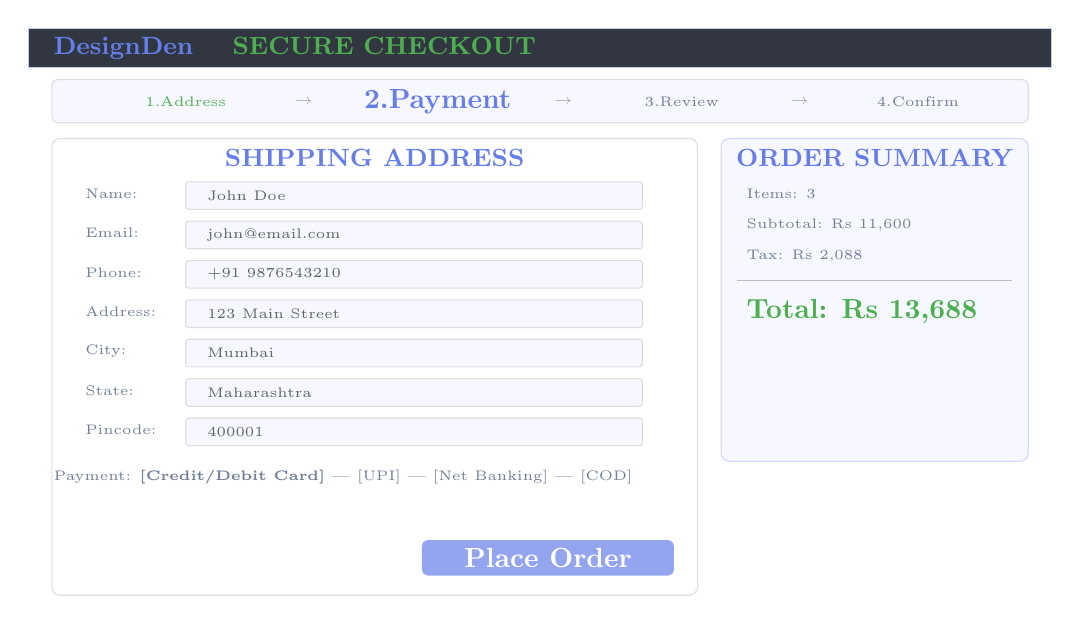
\begin{tikzpicture}[every node/.style={font=\tiny}]
  \filldraw[fill=dark!90, draw=primary!40] (0,7.0) rectangle (13,7.5);
  \node[anchor=west, text=primary, font=\small\bfseries] at (0.2,7.25)
    {DesignDen \quad \textcolor{success}{SECURE CHECKOUT}};

  % Steps bar
  \filldraw[fill=lightbg, draw=dark!15, rounded corners=2pt] (0.3,6.3) rectangle (12.7,6.85);
  \node[text=success] at (2.0,6.57) {1.Address \checkmark};
  \node[text=dark!40] at (3.5,6.57) {$\to$};
  \node[text=primary, font=\bfseries] at (5.2,6.57) {2.Payment};
  \node[text=dark!40] at (6.8,6.57) {$\to$};
  \node[text=muted] at (8.3,6.57) {3.Review};
  \node[text=dark!40] at (9.8,6.57) {$\to$};
  \node[text=muted] at (11.3,6.57) {4.Confirm};

  % Address form
  \filldraw[fill=white, draw=dark!15, rounded corners=3pt] (0.3,0.3) rectangle (8.5,6.1);
  \node[font=\small\bfseries, text=primary] at (4.4,5.85) {SHIPPING ADDRESS};
  \foreach \y/\lbl/\val in {
    5.4/Name:/John Doe,
    4.9/Email:/john@email.com,
    4.4/Phone:/+91\ 9876543210,
    3.9/Address:/123\ Main\ Street,
    3.4/City:/Mumbai,
    2.9/State:/Maharashtra,
    2.4/Pincode:/400001
  }{
    \node[text=muted, anchor=west] at (0.6,\y) {\lbl};
    \filldraw[fill=lightbg, draw=dark!15, rounded corners=1pt] (2.0,\y-0.2) rectangle (7.8,\y+0.15);
    \node[text=dark!70, anchor=west] at (2.15,\y-0.025) {\val};
  }
  \node[text=muted] at (4.0,1.8) {Payment: \textbf{[Credit/Debit Card]} | [UPI] | [Net Banking] | [COD]};
  \filldraw[fill=primary!70, draw=none, rounded corners=2pt] (5.0,0.55) rectangle (8.2,1.0);
  \node[text=white, font=\bfseries] at (6.6,0.775) {Place Order};

  % Order summary
  \filldraw[fill=lightbg, draw=primary!30, rounded corners=3pt] (8.8,2.0) rectangle (12.7,6.1);
  \node[font=\small\bfseries, text=primary] at (10.75,5.85) {ORDER SUMMARY};
  \node[text=muted, anchor=west] at (9.0,5.4) {Items: 3};
  \node[text=muted, anchor=west] at (9.0,5.0) {Subtotal: Rs 11,600};
  \node[text=muted, anchor=west] at (9.0,4.6) {Tax: Rs 2,088};
  \draw[dark!30] (9.0,4.3) -- (12.5,4.3);
  \node[text=success, font=\bfseries, anchor=west] at (9.0,3.9) {Total: Rs 13,688};
\end{tikzpicture}
\end{center}
\end{wireframe}

% ─── Screen 5 ────────────────────────────────────────────────
\subsection{Screen 5 — Designer Dashboard}

\begin{wireframe}{designden.com/designer/dashboard}
\begin{center}
\begin{tikzpicture}[every node/.style={font=\tiny}]
  \filldraw[fill=dark!90, draw=primary!40] (0,7.8) rectangle (13,8.3);
  \node[anchor=west, text=primary, font=\small\bfseries] at (0.2,8.05) {DesignDen  Designer Dashboard};
  \node[anchor=east, text=white!70] at (12.8,8.05) {[Profile v]};

  \node[anchor=west, font=\small\bfseries, text=dark] at (0.3,7.55) {Welcome back, Sarah Designer!};

  % Stats
  \foreach \x/\val/\lbl/\col in {
    0.3/12/Total Orders/primary,
    3.5/8/Active Orders/info,
    6.7/4/Pending Approval/warning,
    9.9/Rs 45.2K/This Month/success
  }{
    \filldraw[fill=white, draw=dark!15, rounded corners=3pt] (\x,5.9) rectangle (\x+2.8,7.2);
    \node[font=\Large\bfseries, text=\col] at (\x+1.4, 6.8) {\val};
    \node[text=muted] at (\x+1.4, 6.4) {\lbl};
  }

  % Tabs
  \filldraw[fill=lightbg, draw=dark!10, rounded corners=2pt] (0.3,5.3) rectangle (12.7,5.75);
  \foreach \i/\t in {1/Orders,2/Portfolio,3/Earnings,4/Messages,5/Settings}{
    \pgfmathsetmacro\x{0.3 + (\i-1)*2.48}
    \ifnum\i=1
      \filldraw[fill=primary!70, draw=none, rounded corners=1pt]
        (\x+0.05,5.35) rectangle (\x+2.38,5.7);
      \node[text=white, font=\bfseries] at (\x+1.2,5.525) {\t};
    \else
      \node[text=muted] at (\x+1.2,5.525) {\t};
    \fi
  }

  % Order cards
  \foreach \y/\id/\status/\scol in {
    3.9/DD-20260215-0042/DESIGN IN PROGRESS/info,
    2.4/DD-20260214-0035/DESIGNER ACCEPTED/primary,
    0.9/DD-20260215-0048/ASSIGNED TO DESIGNER/warning
  }{
    \filldraw[fill=white, draw=dark!15, rounded corners=2pt]
      (0.3,\y-0.3) rectangle (12.7,\y+1.1);
    \node[anchor=west, font=\bfseries, text=dark] at (0.6,\y+0.7) {Order \#\id};
    \filldraw[fill=\scol!15, draw=\scol!40, rounded corners=9pt]
      (8.5,\y+0.5) rectangle (12.5,\y+0.9);
    \node[text=\scol, font=\bfseries] at (10.5,\y+0.7) {\status};
  }
\end{tikzpicture}
\end{center}
\end{wireframe}

% ─── Screen 6 ────────────────────────────────────────────────
\subsection{Screen 6 — Manager Dashboard}

\begin{wireframe}{designden.com/manager/dashboard}
\begin{center}
\begin{tikzpicture}[every node/.style={font=\tiny}]
  \filldraw[fill=dark!90, draw=primary!40] (0,7.8) rectangle (13,8.3);
  \node[anchor=west, text=primary, font=\small\bfseries] at (0.2,8.05) {DesignDen  Manager Dashboard};
  \node[anchor=east, text=white!70] at (12.8,8.05) {[Admin v]};
  \node[anchor=west, text=muted] at (0.3,7.55) {Manager Control Panel -- Production \& Delivery};

  % Stats
  \foreach \x/\val/\lbl/\col in {
    0.3/45/Total Orders/primary,
    3.5/18/Pending Assign/warning,
    6.7/12/In Production/info,
    9.9/8/Ready Delivery/success
  }{
    \filldraw[fill=white, draw=dark!15, rounded corners=3pt] (\x,5.9) rectangle (\x+2.8,7.2);
    \node[font=\Large\bfseries, text=\col] at (\x+1.4, 6.8) {\val};
    \node[text=muted] at (\x+1.4, 6.4) {\lbl};
  }

  % Tabs
  \filldraw[fill=lightbg, draw=dark!10, rounded corners=2pt] (0.3,5.3) rectangle (12.7,5.75);
  \foreach \i/\t in {1/All\ Orders,2/Pending,3/Production,4/Delivery,5/Approval,6/Payouts}{
    \pgfmathsetmacro\x{0.3 + (\i-1)*2.06}
    \ifnum\i=1
      \filldraw[fill=primary!70, draw=none, rounded corners=1pt]
        (\x+0.04,5.35) rectangle (\x+2.0,5.7);
      \node[text=white, font=\bfseries] at (\x+1.0,5.525) {\t};
    \else
      \node[text=muted] at (\x+1.0,5.525) {\t};
    \fi
  }

  % Content cards
  \foreach \y/\title/\status/\scol in {
    3.8/PENDING DESIGN APPROVAL/DESIGN READY/warning,
    2.2/PRODUCTION IN PROGRESS/STITCHING 50\%/info,
    0.7/READY FOR DELIVERY/PRODUCTION COMPLETED/success
  }{
    \filldraw[fill=white, draw=dark!15, rounded corners=2pt]
      (0.3,\y-0.2) rectangle (12.7,\y+1.1);
    \node[anchor=west, font=\bfseries, text=dark] at (0.6,\y+0.75) {\title};
    \filldraw[fill=\scol!15, draw=\scol!40, rounded corners=9pt]
      (8.5,\y+0.5) rectangle (12.5,\y+0.9);
    \node[text=\scol, font=\bfseries] at (10.5,\y+0.7) {\status};
  }
\end{tikzpicture}
\end{center}
\end{wireframe}

% ─── Screen 7 ────────────────────────────────────────────────
\subsection{Screen 7 — Admin Analytics Dashboard}

\begin{wireframe}{designden.com/admin/analytics}
\begin{center}
\begin{tikzpicture}[every node/.style={font=\tiny}]
  \filldraw[fill=dark!90, draw=primary!40] (0,7.8) rectangle (13,8.3);
  \node[anchor=west, text=primary, font=\small\bfseries] at (0.2,8.05) {DesignDen  Admin Analytics};
  \node[anchor=east, text=white!70] at (12.8,8.05) {Super Admin};

  % Stats
  \foreach \x/\val/\lbl/\change/\col in {
    0.3/Rs 2.5L/Revenue/+15\%/primary,
    3.5/342/Orders/+22\%/info,
    6.7/28/Designers/+8\%/secondary,
    9.9/156/Customers/+35\%/warning
  }{
    \filldraw[fill=white, draw=dark!15, rounded corners=3pt] (\x,5.9) rectangle (\x+2.8,7.2);
    \node[font=\large\bfseries, text=\col] at (\x+1.4, 6.75) {\val};
    \node[text=muted] at (\x+1.4, 6.4) {\lbl};
    \node[text=success, font=\bfseries] at (\x+1.4, 6.1) {\change};
  }

  % Revenue chart
  \filldraw[fill=lightbg, draw=dark!15, rounded corners=3pt] (0.3,2.1) rectangle (12.7,5.7);
  \node[font=\small\bfseries, text=primary] at (6.5,5.5) {REVENUE TREND};
  \draw[dark!30, ->] (0.8,2.4) -- (0.8,5.2);
  \draw[dark!30, ->] (0.8,2.4) -- (12.5,2.4);
  % bars
  \foreach \i/\h in {1/1.2, 2/1.5, 3/1.35, 4/1.8, 5/1.65, 6/2.2, 7/1.9, 8/2.1, 9/1.75, 10/2.4}{
    \pgfmathsetmacro\bx{0.8 + (\i-0.5)*1.17}
    \filldraw[fill=primary!60, draw=none, rounded corners=1pt]
      (\bx-0.35,2.4) rectangle (\bx+0.35,{2.4+\h});
  }

  % Pending approvals
  \filldraw[fill=white, draw=dark!15, rounded corners=2pt] (0.3,0.3) rectangle (12.7,1.9);
  \node[anchor=west, font=\small\bfseries, text=dark] at (0.6,1.65) {PENDING APPROVALS};
  \node[text=muted, anchor=west] at (0.6,1.25) {Designer: Emily Rose -- 5 yrs exp -- 12 portfolio items};
  \node[text=muted, anchor=west] at (0.6,0.75) {Manager: Robert Smith -- 3 yrs exp -- MBA};
\end{tikzpicture}
\end{center}
\end{wireframe}

% ─── Screen 8 ────────────────────────────────────────────────
\subsection{Screen 8 — Order Tracking (Customer View)}

\begin{wireframe}{designden.com/orders/DD-20260215-0042}
\begin{center}
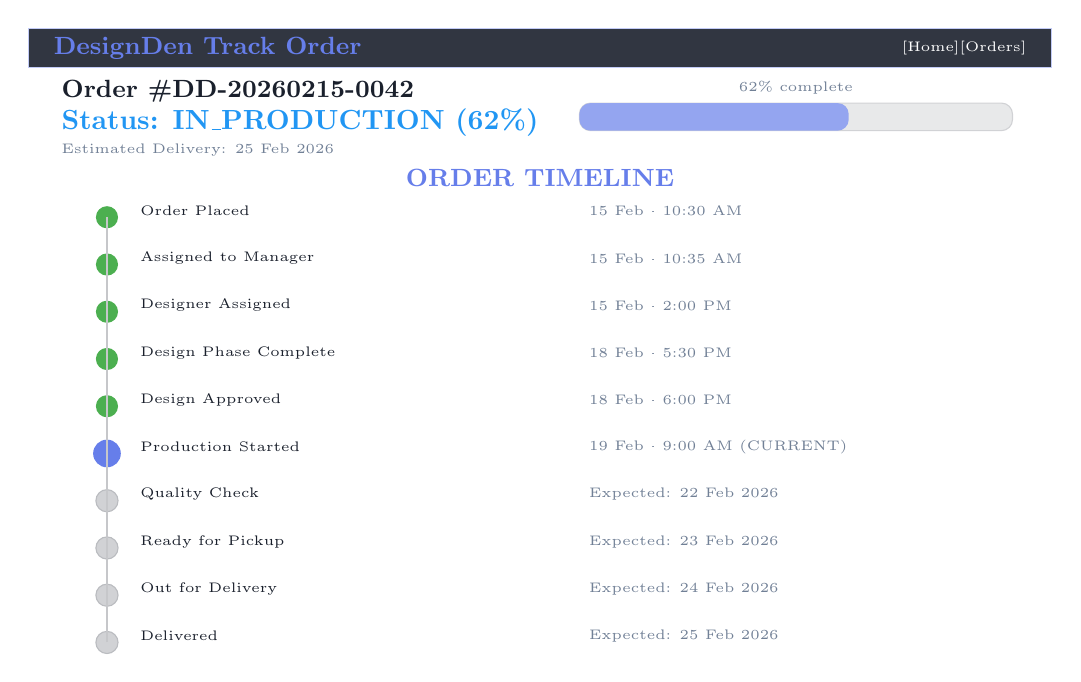
\begin{tikzpicture}[every node/.style={font=\tiny}]
  \filldraw[fill=dark!90, draw=primary!40] (0,7.8) rectangle (13,8.3);
  \node[anchor=west, text=primary, font=\small\bfseries] at (0.2,8.05) {DesignDen  Track Order};
  \node[anchor=east, text=white!70] at (12.8,8.05) {[Home][Orders]};

  \node[anchor=west, font=\small\bfseries, text=dark] at (0.3,7.5) {Order \#DD-20260215-0042};
  \node[anchor=west, text=info, font=\bfseries] at (0.3,7.1) {Status: IN\_PRODUCTION (62\%)};
  \node[anchor=west, text=muted] at (0.3,6.75) {Estimated Delivery: 25 Feb 2026};

  % Progress bar
  \filldraw[fill=dark!10, draw=dark!20, rounded corners=4pt] (7.0,7.0) rectangle (12.5,7.35);
  \filldraw[fill=primary!70, draw=none, rounded corners=4pt] (7.0,7.0) rectangle (10.42,7.35);
  \node[text=muted] at (9.75,7.55) {62\% complete};

  % Timeline
  \node[font=\small\bfseries, text=primary] at (6.5,6.4) {ORDER TIMELINE};
  \foreach \y/\lbl/\date/\done in {
    5.9/Order Placed/15 Feb · 10:30 AM/1,
    5.3/Assigned to Manager/15 Feb · 10:35 AM/1,
    4.7/Designer Assigned/15 Feb · 2:00 PM/1,
    4.1/Design Phase Complete/18 Feb · 5:30 PM/1,
    3.5/Design Approved/18 Feb · 6:00 PM/1,
    2.9/Production Started/19 Feb · 9:00 AM (CURRENT)/2,
    2.3/Quality Check/Expected: 22 Feb 2026/0,
    1.7/Ready for Pickup/Expected: 23 Feb 2026/0,
    1.1/Out for Delivery/Expected: 24 Feb 2026/0,
    0.5/Delivered/Expected: 25 Feb 2026/0
  }{
    \ifnum\done=1
      \filldraw[fill=success, draw=none] (1.0,\y) circle (4pt);
    \else\ifnum\done=2
      \filldraw[fill=primary, draw=none] (1.0,\y) circle (5pt);
    \else
      \filldraw[fill=dark!20, draw=dark!30] (1.0,\y) circle (4pt);
    \fi\fi
    \node[anchor=west, text=dark] at (1.3,\y+0.08) {\lbl};
    \node[anchor=west, text=muted] at (7.0,\y+0.08) {\date};
  }
  % Timeline line
  \draw[dark!25, thick] (1.0,0.5) -- (1.0,5.9);
\end{tikzpicture}
\end{center}
\end{wireframe}

% ─── Screen 9 ────────────────────────────────────────────────
\subsection{Screen 9 — Designer-Customer Chat Interface}

\begin{wireframe}{designden.com/chat/DD-20260215-0042}
\begin{center}
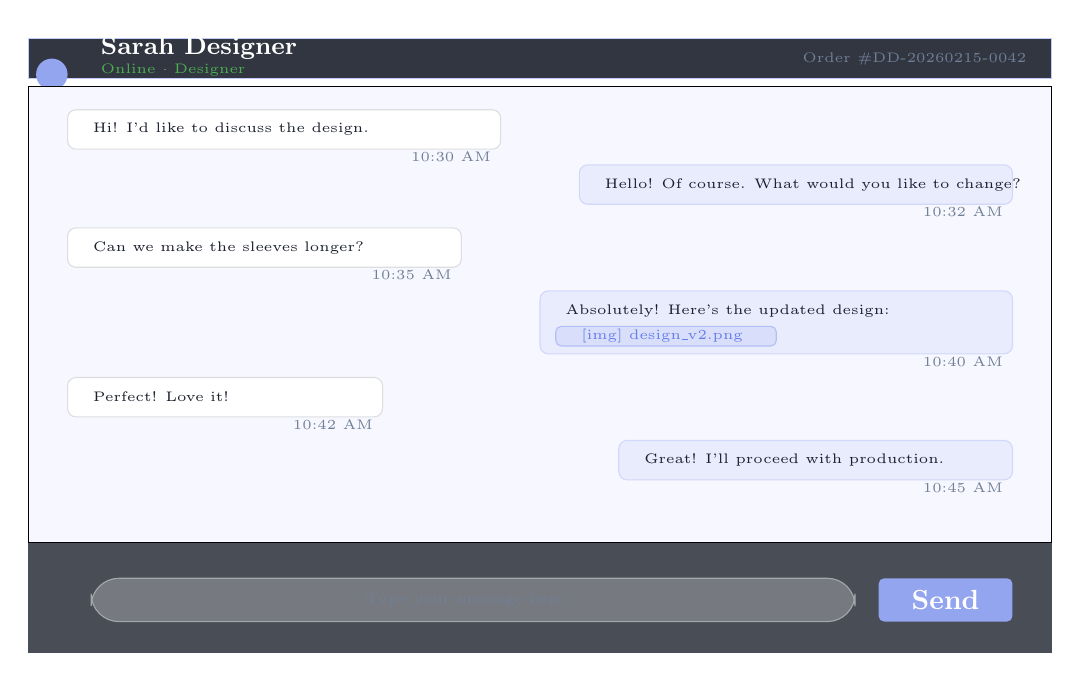
\begin{tikzpicture}[every node/.style={font=\tiny}]
  % Chat header
  \filldraw[fill=dark!90, draw=primary!40] (0,7.3) rectangle (13,7.8);
  \filldraw[fill=primary!70, draw=none] (0.3,7.35) circle (0.2);
  \node[anchor=west, text=white, font=\small\bfseries] at (0.8,7.685) {Sarah Designer};
  \node[text=success, anchor=west] at (0.8,7.4) {Online · Designer};
  \node[text=muted, anchor=east] at (12.8,7.55) {Order \#DD-20260215-0042};

  % Messages
  \filldraw[fill=lightbg] (0,1.4) rectangle (13,7.2);

  % Incoming
  \filldraw[fill=white, draw=dark!15, rounded corners=3pt] (0.5,6.4) rectangle (6.0,6.9);
  \node[anchor=west, text=dark] at (0.7,6.65) {Hi! I'd like to discuss the design.};
  \node[anchor=east, text=muted] at (6.0,6.3) {10:30 AM \checkmark\checkmark};

  % Outgoing
  \filldraw[fill=primary!15, draw=primary!30, rounded corners=3pt] (7.0,5.7) rectangle (12.5,6.2);
  \node[anchor=west, text=dark] at (7.2,5.95) {Hello! Of course. What would you like to change?};
  \node[anchor=east, text=muted] at (12.5,5.6) {10:32 AM \checkmark\checkmark};

  % Incoming
  \filldraw[fill=white, draw=dark!15, rounded corners=3pt] (0.5,4.9) rectangle (5.5,5.4);
  \node[anchor=west, text=dark] at (0.7,5.15) {Can we make the sleeves longer?};
  \node[anchor=east, text=muted] at (5.5,4.8) {10:35 AM \checkmark\checkmark};

  % Outgoing with attachment
  \filldraw[fill=primary!15, draw=primary!30, rounded corners=3pt] (6.5,3.8) rectangle (12.5,4.6);
  \node[anchor=west, text=dark] at (6.7,4.35) {Absolutely! Here's the updated design:};
  \filldraw[fill=primary!25, draw=primary!50, rounded corners=2pt] (6.7,3.9) rectangle (9.5,4.15);
  \node[text=primary, anchor=west] at (6.9,4.025) {[img] design\_v2.png};
  \node[anchor=east, text=muted] at (12.5,3.7) {10:40 AM \checkmark\checkmark};

  % Incoming
  \filldraw[fill=white, draw=dark!15, rounded corners=3pt] (0.5,3.0) rectangle (4.5,3.5);
  \node[anchor=west, text=dark] at (0.7,3.25) {Perfect! Love it!};
  \node[anchor=east, text=muted] at (4.5,2.9) {10:42 AM \checkmark\checkmark};

  % Outgoing
  \filldraw[fill=primary!15, draw=primary!30, rounded corners=3pt] (7.5,2.2) rectangle (12.5,2.7);
  \node[anchor=west, text=dark] at (7.7,2.45) {Great! I'll proceed with production.};
  \node[anchor=east, text=muted] at (12.5,2.1) {10:45 AM \checkmark};

  % Input row
  \filldraw[fill=dark!80, draw=none] (0,0) rectangle (13,1.4);
  \filldraw[fill=dark!60, draw=dark!40, rounded corners=10pt] (0.8,0.4) rectangle (10.5,0.95);
  \node[text=muted] at (5.65,0.675) {Type your message here...};
  \filldraw[fill=primary!70, draw=none, rounded corners=2pt] (10.8,0.4) rectangle (12.5,0.95);
  \node[text=white, font=\bfseries] at (11.65,0.675) {Send};
\end{tikzpicture}
\end{center}
\end{wireframe}

% ─────────────────────────────────────────────────────────────
\section{Common UI Patterns}

\subsection{Navigation Bar Structure}

\begin{mdframed}[linecolor=primary!40, backgroundcolor=primary!4]
\begin{tabular}{@{}L{3cm}L{4cm}L{6cm}@{}}
\toprule
\rowcolor{tabhead}
\textbf{Element} & \textbf{Content} & \textbf{Behaviour} \\
\midrule
Logo          & ``DesignDen'' (gradient) & Links to \texttt{/} \\
Nav Links     & Role-dependent menu items & Highlight active route \\
Cart Badge    & Item count               & Animated on add \\
Profile Menu  & Dropdown with role links & Role-based options \\
Auth Buttons  & Login / Logout           & Toggle on auth state \\
\bottomrule
\end{tabular}
\end{mdframed}

\subsection{Card Pattern}
\begin{lstlisting}
┌────────────────────────────┐
│  [Icon]  Title             │
│  ─────────────────────     │
│  Description text goes     │
│  here with details.        │
│                            │
│  [Action Button]           │
└────────────────────────────┘
\end{lstlisting}

\subsection{Timeline Pattern}
\begin{lstlisting}
[✓] Event 1 (done)        Date/time
 |
[✓] Event 2 (done)        Date/time
 |
[●] Event 3 (current)     Date/time  ← animated pulse
 |
[○] Event 4 (future)      Expected date
 |
[○] Event 5 (future)      Expected date
\end{lstlisting}

\subsection{Progress Bar Pattern}
\begin{lstlisting}
  [▰▰▰▰▰▰▱▱▱▱]  62%
  gradient: #667eea → #764ba2
\end{lstlisting}

\vfill
\begin{center}
  \small\textcolor{muted}{DesignDen $\cdot$ Wireframes \& UI $\cdot$ v1.0 $\cdot$ March 2026}
\end{center}

\end{document}
